\chapter{Resultados y discusión}\label{chapter:resultados}

Aquí se discutirán los resultados, tablas de datos y gráficas.

Por ejemplo, la Tabla \ref{tab:mi-tabla-grande}, muestra un ejemplo de como introducir tablas de forma limpia en el texto.

\begin{table}[htbp!] % Posición de la tabla en la página
\centering % Centrar la tabla
\caption[Tabla grande]{Mi tabla grande con cabeceras en negrita}
\label{tab:mi-tabla-grande} % Etiqueta de referencia para la tabla

\begin{tabular}{@{}lrrr@{}}
\toprule
\textbf{Categoría} & \textbf{Valor 1} & \textbf{Valor 2} & \textbf{Valor 3} \\ \midrule
Fruta 1 & 5 & 10 & 15 \\
Fruta 2 & 8 & 12 & 18 \\
Verdura 1 & 3 & 6 & 9 \\
Verdura 2 & 4 & 7 & 11 \\
Bebida 1 & 1 & 2 & 3 \\
Bebida 2 & 6 & 9 & 12 \\ \bottomrule
\end{tabular}
\end{table}



Fíjate que tanto tablas como imágenes, deben estar previamente referenciadas en el texto, y no deben separarse mucho de éste. Fíjate también en como se crean títulos reducidos para que el texto del pie de tabla no ocupe demasiado en el índice.

Las tablas enormes como la Tabla \ref{tab:mi-tabla-enorme}, deben intentar colocarse en una página aparte.

\begin{sidewaystable}[htbp] % Rotar la tabla 90 grados
\centering
\caption[Tabla enorme]{Mi tabla enorme de población}
\label{tab:mi-tabla-enorme} % Etiqueta de referencia para la tabla

\begin{tabular}{clrrrrrrrrc}
\toprule
\textbf{Categoría} & \textbf{Valor 1} & \textbf{Valor 2} & \textbf{Valor 3} & \textbf{Valor 4} & \textbf{Valor 5} & \textbf{Valor 6} & \textbf{Valor 7} & \textbf{Valor 8} & \textbf{Valor 9} & \textbf{Valor 10} \\ \midrule
Ecuador & 5 & 10 & 15 & 20 & 25 & 30 & 35 & 40 & 45 \\
Nicaragua & 8 & 12 & 18 & 24 & 30 & 36 & 42 & 48 & 54 \\
Honduras & 3 & 6 & 9 & 12 & 15 & 18 & 21 & 24 & 27 \\
Argentina & 4 & 7 & 11 & 15 & 19 & 23 & 27 & 31 & 35 \\
Venezuela & 1 & 2 & 3 & 4 & 5 & 6 & 7 & 8 & 9 \\
Colombia & 6 & 9 & 12 & 15 & 18 & 21 & 24 & 27 & 30 \\
Chile & 2 & 4 & 6 & 8 & 10 & 12 & 14 & 16 & 18 \\
España & 7 & 11 & 15 & 19 & 23 & 27 & 31 & 35 & 39 \\
% Agrega más filas según sea necesario hasta 30 filas
\bottomrule
\end{tabular}

\end{sidewaystable}



Lo mismo se puede hacer con las gráficas. Pero ten cuidado de que las gráficas no se vayan lejos del texto tampoco. Vamos a poner un ejemplo para que no nos moleste la tabla anterior, vamos a forzar una nueva página.

\newpage

Se deben evitar imágenes ``por poner''\footnote{Por cierto, fíjate en cómo van las comillas. Aunque es mejor usar cursivas. Las palabras en inglés, por ejemplo, deberían ir en \emph{cursiva}, como por ejemplo \emph{buffer}.}, como la Figura \ref{fig:logo}. Que es un logotipo. 

\begin{figure}[htb!] % Posición de la figura en la página
\centering % Centrar la figura

\includegraphics[width=0.5\textwidth]{logo} % Reemplaza "logo.png" con la ruta a tu imagen
\caption{Mi logo}
\label{fig:logo} % Etiqueta de referencia para la figura
\end{figure}


Por ejemplo, la Figura \ref{fig:grafica} sí que está correcta, y va de la misma forma que la tabla, y ahora está cerca del texto. Hemos sacrificado un poco de espacio al final de la página anterior a cambio de acercar la figura al texto. Esto solo debe hacerse en casos en que tengamos tablas y figuras que ocupen la página completa.

\begin{figure}[htb!] % Posición de la figura en la página
\centering % Centrar la figura
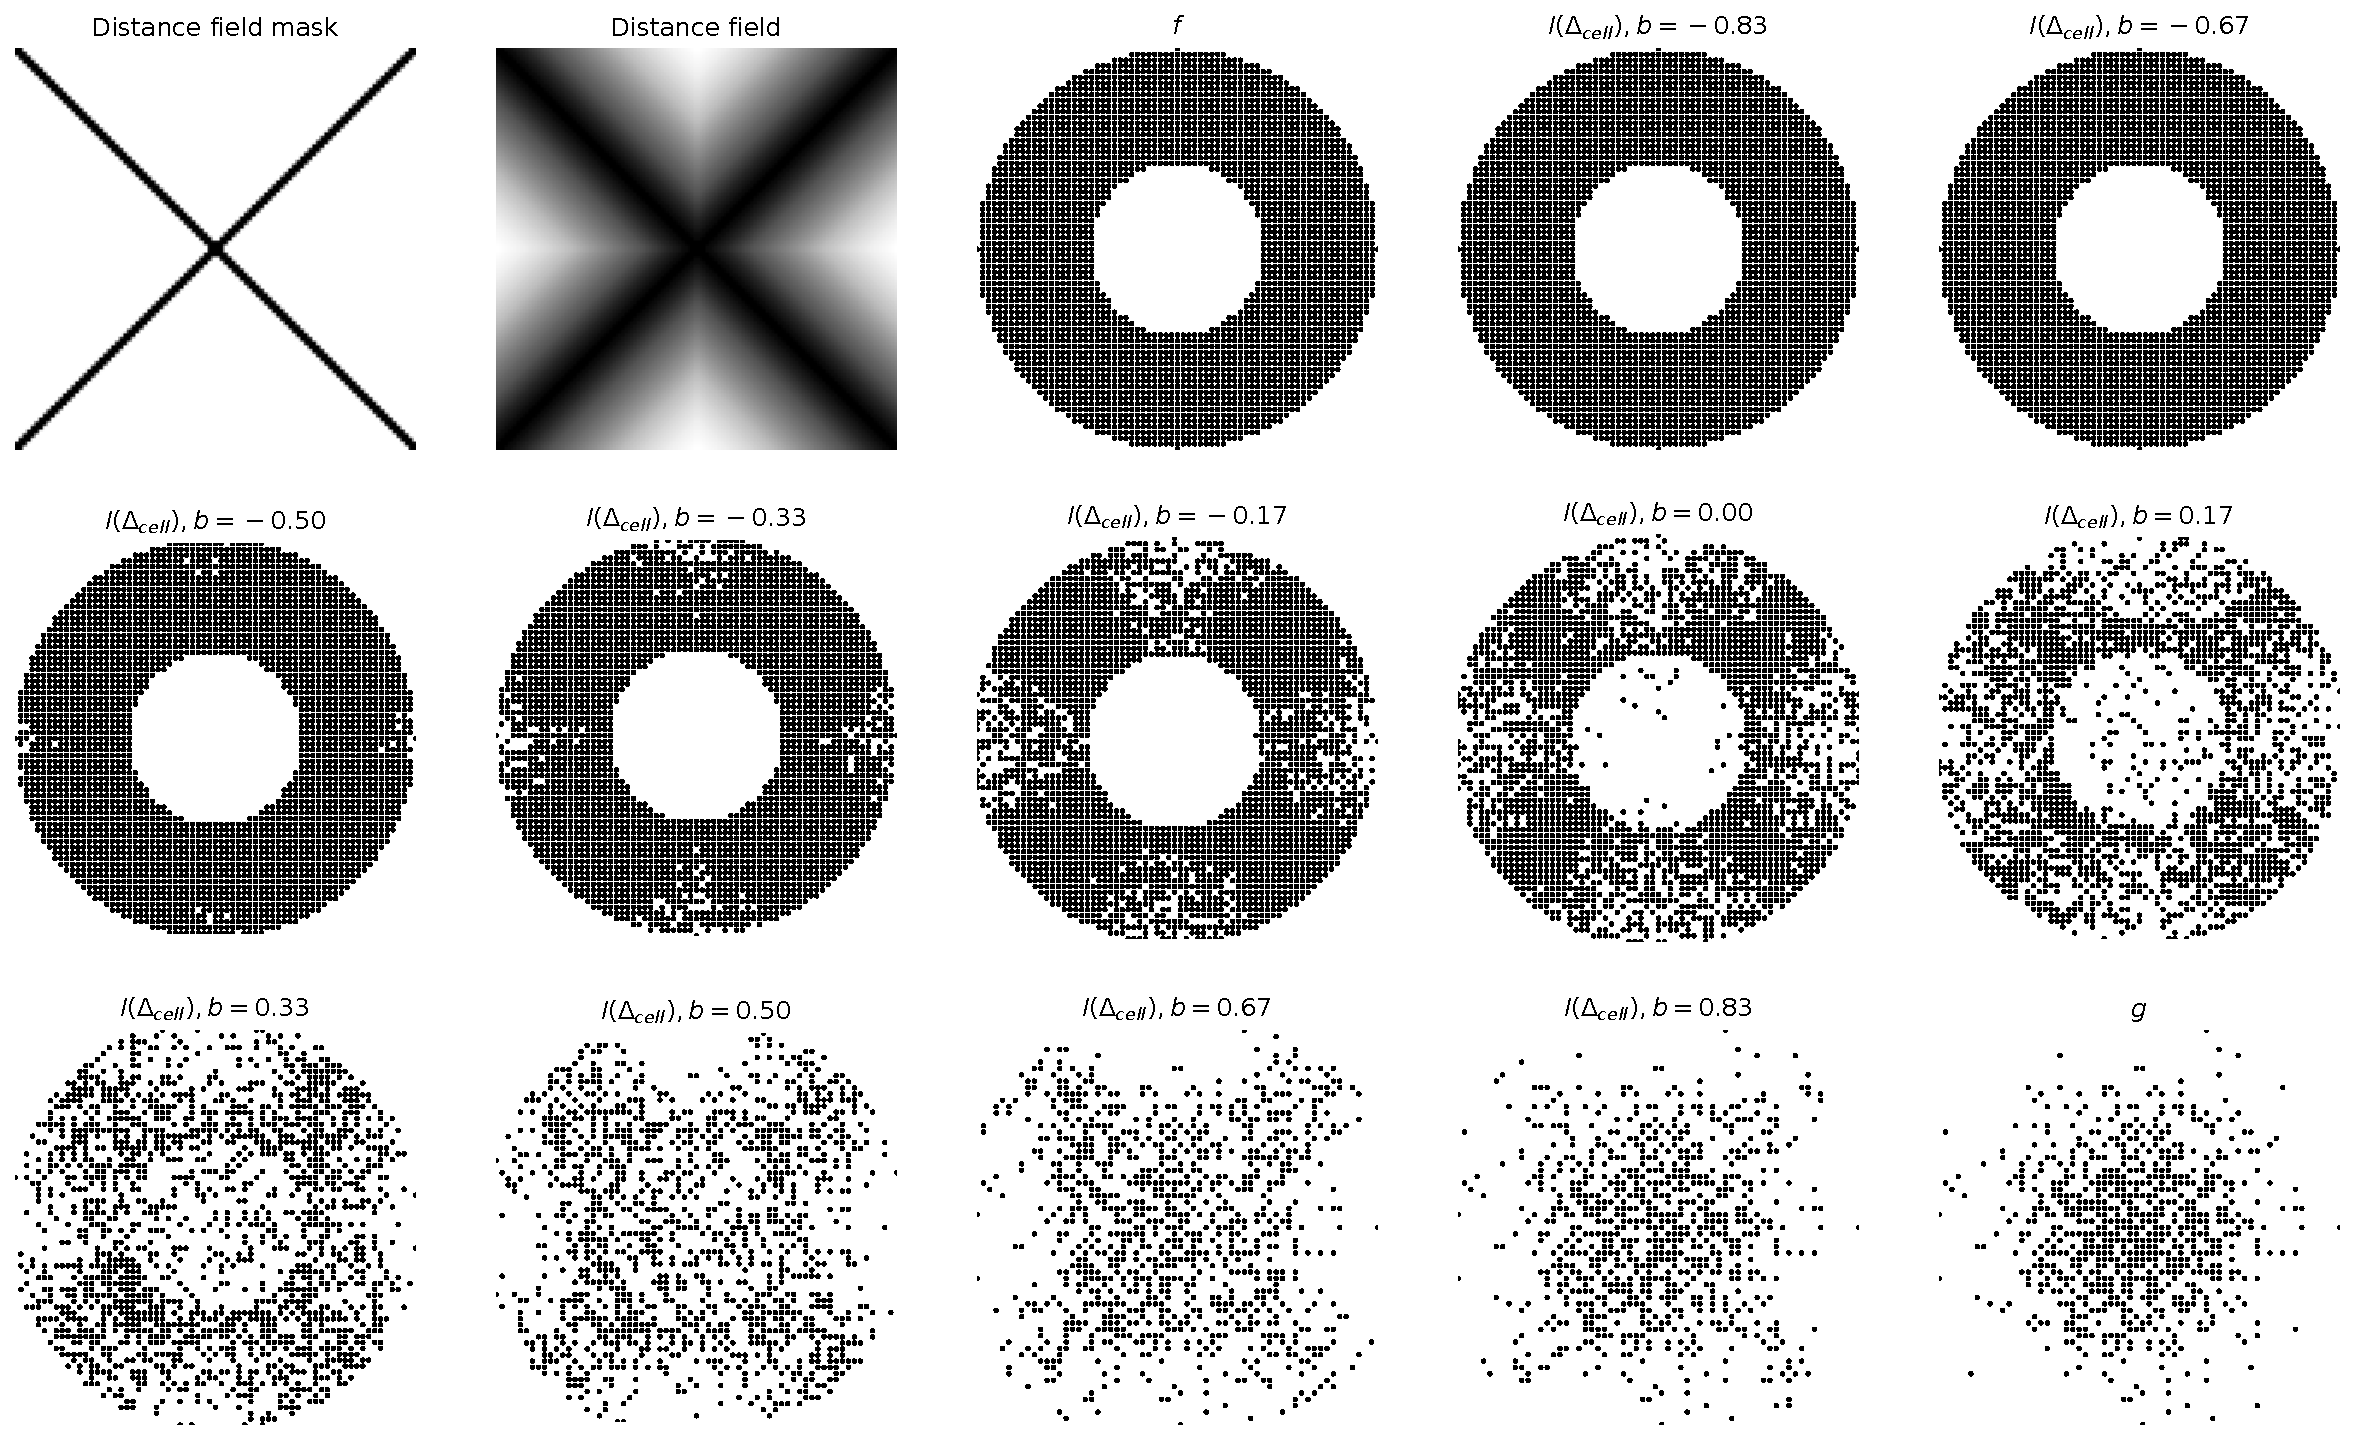
\includegraphics[width=\textwidth]{test-distribuciones}
\caption[Lista de distribuciones]{Lista de distribuciones: Aquí iría una descripción de la figura para cada fila o columna, explicando los parámetros. Fíjate como el pie está recortado en el índice para que no sea extremadamente largo. Si hay una fuente, la podemos colocar aquí: \url{https://drive.google.com/file/d/14YN87TAF6OQq6JIuZiUz3YHn-6Pz8KHm/view?usp=sharing}}
\label{fig:grafica} % Etiqueta de referencia para la figura
\end{figure}


El tipo de extensiones ya está definido, así que no deben usarse a la hora de referenciar imágenes. Por defecto el orden es:

\begin{enumerate}
    \item PDF: Son gráficos vectoriales con máxima calidad, bueno para esquemas y tablas.
    \item PNG: Son gráficos que no pierden calidad, aunque son gráficos \emph{raster} o matriciales. Utilízalos cuando los tonos sean planos, como en esquemas, en sustitución de los PDF cuando no tenemos opción a usar gráficos vectoriales.
    \item JPEG: Con extensión \textbf{.jpg}, se suelen usar cuando son fotografías, principalmente, ya que pueden contener \emph{artifacts}.
\end{enumerate}